\documentclass[tikz,border=0pt]{standalone}
\usepackage[utf8]{inputenc}
\usepackage[T1]{fontenc}
\usepackage{lmodern}
\usepackage{amsmath,amssymb}
\usetikzlibrary{arrows.meta,positioning,fit,calc,backgrounds,shapes.geometric,decorations.pathreplacing}
\definecolor{navy}{HTML}{163A5F}
\definecolor{blue}{HTML}{2C6EAF}
\definecolor{lightblue}{HTML}{EAF2F8}
\definecolor{midblue}{HTML}{CFE1F2}
\definecolor{graytext}{HTML}{4A5560}
\definecolor{lightgray}{HTML}{F4F6F8}
\definecolor{green}{HTML}{3C8D73}
\definecolor{lightgreen}{HTML}{E8F5EF}
\definecolor{red}{HTML}{B24A4A}
\definecolor{lightred}{HTML}{FBEDEE}
\tikzset{
  title/.style={font=\sffamily\bfseries\fontsize{16}{18}\selectfont,text=navy,anchor=west},
  subtitle/.style={font=\sffamily\bfseries\fontsize{11}{13}\selectfont,text=navy},
  body/.style={font=\sffamily\fontsize{9.2}{11}\selectfont,text=graytext,align=left},
  small/.style={font=\sffamily\fontsize{8}{9.4}\selectfont,text=graytext,align=left},
  tinylabel/.style={font=\sffamily\fontsize{7.2}{8.4}\selectfont,text=graytext},
  panel/.style={rounded corners=3pt,draw=midblue,fill=white,line width=0.6pt},
  box/.style={rounded corners=2pt,draw=midblue,fill=lightblue,line width=0.6pt},
  worker/.style={rounded corners=2pt,draw=blue,dashed,line width=0.7pt,fill=white},
  task/.style={rounded corners=2pt,draw=blue,fill=lightblue,minimum width=0.85cm,minimum height=0.55cm,font=\sffamily\bfseries\small,text=navy},
  file/.style={draw=blue,fill=white,minimum width=0.55cm,minimum height=0.42cm,font=\sffamily\small,text=navy},
  arr/.style={-{Stealth[length=2.4mm,width=1.8mm]},draw=blue,line width=0.9pt},
  arrthin/.style={-{Stealth[length=2mm,width=1.5mm]},draw=blue,line width=0.7pt},
  arrred/.style={-{Stealth[length=2mm,width=1.5mm]},draw=red,dashed,line width=0.8pt},
  arrgreen/.style={-{Stealth[length=2mm,width=1.5mm]},draw=green,dotted,line width=1pt}
}
\begin{document}

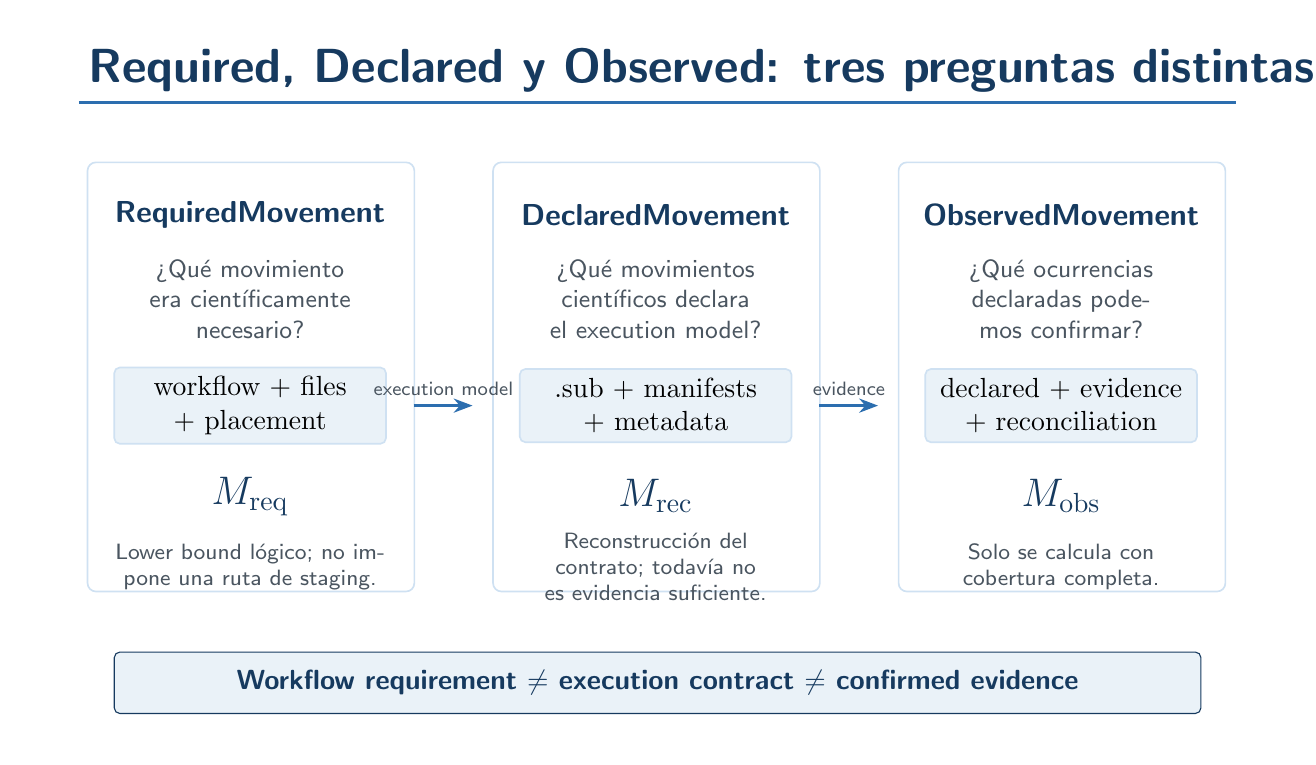
\begin{tikzpicture}[x=1cm,y=1cm]
\path[use as bounding box] (0,0) rectangle (16,9);
\node[title] at (0.65,8.45) {Required, Declared y Observed: tres preguntas distintas};
\draw[blue,line width=1pt] (0.65,8.05)--(15.35,8.05);
\foreach \x/\ttl/\q/\src/\sym/\note in {
0.75/{RequiredMovement}/{¿Qué movimiento era científicamente necesario?}/{workflow + files + placement}/{$M_{\mathrm{req}}$}/{Lower bound lógico; no impone una ruta de staging.},
5.9/{DeclaredMovement}/{¿Qué movimientos científicos declara el execution model?}/{.sub + manifests + metadata}/{$M_{\mathrm{rec}}$}/{Reconstrucción del contrato; todavía no es evidencia suficiente.},
11.05/{ObservedMovement}/{¿Qué ocurrencias declaradas podemos confirmar?}/{declared + evidence + reconciliation}/{$M_{\mathrm{obs}}$}/{Solo se calcula con cobertura completa.}}
{
\node[panel,minimum width=4.15cm,minimum height=5.45cm,anchor=north west] at (\x,7.3) {};
\node[subtitle,text width=3.6cm,align=center] at (\x+2.075,6.62) {\ttl};
\node[body,text width=3.5cm,align=center] at (\x+2.075,5.55) {\q};
\node[box,minimum width=3.45cm,minimum height=0.85cm,text width=3.1cm,align=center] at (\x+2.075,4.2) {\src};
\node[font=\sffamily\bfseries\Large,text=navy] at (\x+2.075,3.05) {\sym};
\node[small,text width=3.45cm,align=center] at (\x+2.075,2.15) {\note};
}
\draw[arr] (4.9,4.2)--(5.65,4.2); \node[tinylabel,above] at (5.28,4.2) {execution model};
\draw[arr] (10.05,4.2)--(10.8,4.2); \node[tinylabel,above] at (10.43,4.2) {evidence};
\node[rounded corners=2pt,draw=navy,fill=lightblue,minimum width=13.8cm,minimum height=0.78cm,font=\sffamily\bfseries,text=navy] at (8,0.68) {Workflow requirement $\neq$ execution contract $\neq$ confirmed evidence};
\end{tikzpicture}
\end{document}
